%% $RCSfile: proj_report_outline.tex,v $
%% $Revision: 1.2 $
%% $Date: 2010/04/23 02:40:16 $
%% $Author: kevin $

\documentclass[11pt
              , a4paper
              , twoside
              , openright
              ]{report}


\usepackage{float} % lets you have non-floating floats

\usepackage{url} % for typesetting urls
\usepackage[numbers]{natbib}

%
%  We don't want figures to float so we define
%
\newfloat{fig}{thp}{lof}[chapter]
\floatname{fig}{Figure}

%% These are standard LaTeX definitions for the document
%%                            
\title{PitchHub - A Collaboration Platform for Innovators}
\author{Michael Winton}

%% This file can be used for creating a wide range of reports
%%  across various Schools
%%
%% Set up some things, mostly for the front page, for your specific document
%
% Current options are:
% [ecs|msor]              Which school you are in.
%
% [bschonscomp|mcompsci]  Which degree you are doing
%                          You can also specify any other degree by name
%                          (see below)
% [font|image]            Use a font or an image for the VUW logo
%                          The font option will only work on ECS systems
%
\usepackage[image,ecs,mcompsci]{vuwproject}

\usepackage{graphicx}
\usepackage{wrapfig}
\usepackage{lscape}
\usepackage{rotating}
\graphicspath{ {images/} }

% font
% You should specifiy your supervisor here with
\supervisor{Dr. Kris Bubendorfer}
% use \supervisors if there is more than one supervisor

% Unless you've used the bschonscomp or mcompsci
%  options above use
\otherdegree{ENGR489 - Bachelor of Engineering}
% here to specify degree

% Comment this out if you want the date printed.
\date{}

\begin{document}

% Make the page numbering roman, until after the contents, etc.
\frontmatter

%%%%%%%%%%%%%%%%%%%%%%%%%%%%%%%%%%%%%%%%%%%%%%%%%%%%%%%

%%%%%%%%%%%%%%%%%%%%%%%%%%%%%%%%%%%%%%%%%%%%%%%%%%%%%%%

\begin{abstract}

The ability to connect innovative ideas to people and resources is an essential component of the innovation process. This project is concerned with empowering the innovation community with an online collaboration system that is simultaneously useful to all actors in the innovation ecosystem while ensuring that all sensitive IP shared is stored in a secure manner. The goal of this report is to detail the steps taken in designing and implementing a distributed web application that facilitates collaboration and enforces data security with threshold cryptography.

\end{abstract}

%%%%%%%%%%%%%%%%%%%%%%%%%%%%%%%%%%%%%%%%%%%%%%%%%%%%%%%

\maketitle

% %!TEX root = proj_report_outline.tex
\chapter*{Acknowledgements}\label{C:ack} 

\begin{chapquote}{Franklin D. Roosevelt}
``Happiness lies in the joy of achievement and the thrill of creative effort.''
\end{chapquote}

\noindent
I would like to acknowledge the people who have helped me throughout this year. 
\\
\newline
Firstly, I would like to express my profound thanks to my supervisor Dr. Kris Bubendorfer, for his continuous support throughout this project. The guidance and advice I have received has been invaluable to this project, and I hope to keep it close in mind moving into the future.
\\
\newline
I would like to thank my friends at Callaghan Innovation: Dr. Gregor Neumayr, Donal Krouse, and Peter McGavin, for their help and direction, but also for the hard questions that ultimately made this project better and more rewarding.
\\
\newline
Additionally, I thank my peers for their willingness to be my sounding board, for the late nights we have shared, and for the last four years of friendship.
\\
\newline
Last but not least, I would like to thank my Mum for her endless support. I hope I made you proud.
\\
\newline
\textit{Michael Winton}

\tableofcontents

% we want a list of the figures we defined
\listof{fig}{Figures}

%%%%%%%%%%%%%%%%%%%%%%%%%%%%%%%%%%%%%%%%%%%%%%%%%%%%%%%

\mainmatter

%%%%%%%%%%%%%%%%%%%%%%%%%%%%%%%%%%%%%%%%%%%%%%%%%%%%%%%

% individual chapters included here

\chapter{Introduction}

\section{Motivation}

\section{Project Objective and Scope}

roles and rights (scope of disclosure)

\section{Contributions}

\section{Outline}
%!TEX root = proj_report_outline.tex
\chapter{Background into Collaborative Platforms for Innovation}

This chapter aims to explore the related works of collaborative platforms used in the innovation space and also contextualises where in this landscape PitchHub aims to occupy. First, this chapter presents a taxonomy of the primary roles used within the collaborative innovation process. Second, this chapter describes the current collaborative platforms being used in the innovation space and establishes where each stands within the role taxonomy. Third, this chapter concludes with a discussion on the practical limitations that are introduced by being innovation-orientated.

\section{Common Roles in Innovation}

The process of driving an idea from its conceptualisation to its realisation commonly requires a variety of actors who bring together the knowledge, skills and resources required to action its fulfillment. For example, the Apple ][ came to being with Steve Wozniak providing the technical knowledge and skills, Steve Jobs providing the project goals and marketing drive, and Mike Markulla providing the resources to finance it's production \cite{livingston2007founders}. Again and again we see similar stories, where innovation is driven in a collaborative configuration rather than solely by one person. To this point Callaghan Innovation has identified four distinct roles that are embodied by the team within the innovation process:

\begin{itemize}
	\item Challenger
	\item Enabler
	\item Solver
	\item Facilitator
\end{itemize}

These four roles represent the different functions required in an innovative product or service's successful execution. Challengers provide the idea or problem to solved in order to realise a business opporunity. Enablers provide the resources required to action the innovation, this may be in terms of man-power, assets or financing. Solvers provide the answer to the idea or problem presented by the Challenger(s). Facilitators provide the connections to drive the innovation's exection, this may be in terms of connecting other people to the idea, or helping the idea gain reputation. Whether these roles are shared amongst a team or fulfilled by a single person in most cases of innovation these roles are too large for one person to embody them all. To continue with the Apple ][ example, we may catergorise Steve Jobs as the challenger, asking why computers can't serve the consumer market, Steve Wozniak can be seen as an enabler and sover, as he both designed the Apple ][ and built them, and Mike Markulla, can be regarded as an enabler and facilitator, as he financed the production and also lent his reputation to the product. 

\section{An Investigation of Collaborative Platforms}
Naturally, a platform that aims to facilitate collaboration for purposes of innovation at it's empowering an idea in relation to these roles. In this section we explore the current solutions being used to facilitate collaboration and discuss how each works in relation to these roles.
\\
\\
\textbf{IdeaForge}\cite{ideaForge:online}
is a collaborative innovation platform that supports the Challenger, Enabler and Solver roles. In it's own parlance IdeaForge is described as a three-sided marketplace where users can provide ``ideas, time/skills or cash/resources". The main aim for this platform is to facilitate anytime/anywhere collaboration within the global innovation community. Additionally, IdeaForge provides some visibility settings for ideas, where they may be scoped as visible publicly or members only. IdeaForge does not provide functionality for Facilitators, therefore ideas being hosted on IdeaForge require external facilitation. IdeaForge can be regarded as the most similar to PitchHub in spirit as it serves many of the roles identified and provides scoping functionality.
\\
\\
\textbf{Assembly}\cite{assembly:online}
is a collaborative platform that implicitly supports Challenger, Enabler, Solver, and Facilitator roles. Assembly is orientated around communities that may focus on one or more ideas. The platform does not explicitly distinguish between the roles identified but it's forum-like structure means that any of these roles may raise challenges or solutions within the groups. Assembly's recommender system functionality, where users get recommended groups they may be interested in, illustrates how Assembly itself can be seen as carrying out the Facilitator's role. PitchHub and Assembly differ on focus, where PitchHub focuses on the idea Assembly focuses on the community, this structure while applicable to the innovation space is less directed towards the immediate fulfillment of ideas and more for general collaboration.
\\
\\
\textbf{AngelList}\cite{Angel:online} and \textbf{Enterprise Angels} are examples of online platforms for investors, a subset of of Enablers, looking to fund businesses. Crowd funding and microequity platforms such as \textbf{Kickstarter}, \textbf{Indiegogo} and \textbf{PledgeMe} are becoming increasingly viable sources of funding. These platforms are primarily for Challenger/Solvers looking to seed their innovations, and Enablers looking to get return on their investment. An interesting phenomenon of these platforms is the social ``hype" that is sometimes garnered around many of the products/services launched on these platforms. While the solicitation of funds is not a primary goal of PitchHub the inherent socialness of these funding platforms is directly comparable.
\\
\\
Inevitably large social networks have also been used in the innovation space as platforms to help facilitate collaboration. Examples include \textbf{LinkedIn} being used by New Zealand Healthcare Innovation, \textbf{Facebook} being used in the Great New Zealand Science Project, and \textbf{Google Groups} being used in the National Science Challenges. These platforms have the inherent benefit of convenience as many people in the innovation ecosystem are already members of these networks. These platforms however suffer from lack of (used) privacy controls, and therefore is not a conducive environment for users wishing to discuss commercially sensitive information. These repurposed examples of social networks are in stark constrast to PitchHub's goal of facilitating collaborative innovation.
\\
\\
The proliferation of online networks has been a boon for communities, enabling unprecedented reach. The innovation community has benefitted greatly from these networks, however as demonstrated in the above investigation these networks lack features which serve the directed making of connections between all roles within the innovation community.

[visualise the above, force directed graph layout?]

PitchHub aims to learn and build on many of the ideas from these networks. First, to provide a platform that serves all roles within the innovation ecosystem. Second, to systematically build valuable business connections centerd around an idea. Third, to enable users privacy control over their contributions to an idea.

\section{Practical Limitations of Online Collaboration for Innovation}
%!TEX root = proj_report_outline.tex

\chapter{Web Application Design}\label{C:design_web}

TODO

The design of the web application focused on the use of standard architecture patterns and web development technologies. This approach was taken as web application development covers numerous domains and technologies. In \citeauthor{shklar2009web}'s tome ``Web Application Architecture: Principles, Protocols and Practices'' they describe the core areas of knowledge required: HTTP, HTML, SMTP, JavaScript, Databases, Graphics Design, and Server Technology \cite{shklar2009web}. While designing a unique foundation specifically optimised for PitchHub is enticing, as Donald Knuth is famously quoted ``97\% of the time premature optimization is the root of all evil'' \cite{knuth1974structured}. With this in mind, PitchHub leverages battle tested open source libraries to deliver more functionality while reserving the ability to make custom modifications and changes as necessary. This chapter explores these design choices and also the alternative designs that were considered throughout this project.

\section{User Stories}

The principal function of PitchHub is to facilitate collaboration in the innovation community, this is reflected in requirement D1. As such the design of PitchHub began with specifying these fundamentals in user stories. To do this each user story captured a desired behaviour by identifying the behaviour's corresponding `who', `what', and `why' attributes. An example user story capturing \textit{Post Pitch Card} behaviour is as follows:

\begin{verbatim}
	  As a user, I want to create a Pitch Card so that the community and I may 
	  collaborate to find a solution	
\end{verbatim}

To unpack on this example, the `who' is a user, the `what' is the ability post Pitch Cards, and the `why' is the desire of finding a solution through collaboration.
So from these user stories not only is the behaviour captured but also relevant expectations of state. To continue using the above example, it can be discerned that once the user has posted a Pitch Card there is an expectation that other users will be able to see it and also interact with it `to find a solution'. Specifying these user stories was done in collaboration with Callaghan Innovation to ensure the behaviour documented was accurate. 

To have a complete understanding of the functionality required by PitchHub user stories were used to describe all desired behaviour, ranging from sign-up to content scoping (as per requirement D2.1). These user stories are found in Appendix \ref{A:user_stories}.

\section{UI Design}

A well-designed user interface drives user behaviour. Given PitchHub's aim of facilitating collaboration behaviour it is advantageous to have it also drive it. Specifically the behaviour aimed to be driven is those found in requirements D1, D2.1, and D2.2. To do this, the behaviour captured in the user stories were embraced in the content templates and wire frames created to guide the final UI design.
The creation of content templates for each page were the first step in UI design. Content templates were used as they place emphasis on the narrative of each page being designed first before the visual elements, thus prioritising the fundamentals. Ultimately, through content templates each page is deconstructed into: who the target audience is, what the page's purpose is, and what the context is. An example content template for the Pitch Card page can be found in Appendix \ref{A:content_template}.
Wire frames were then used to iterate on the layout of each page. This process solely focused on the layout and visual design of each page rather than the content (having already been specified in the content templates).


\section{Architecture}

The architecture of the web application was some of the first work accomplished on PitchHub. The architecture is the abstraction of the system and hence should be designed with the desired system qualities needed to to be achieved. With PitchHub the security and distributed requirements identified in Chapter \ref{C:requirements} were captured in the three tier architecture designed, hence formalising the requirements specification early on.
\par
The common software engineering practice of separation of concerns has a strong presence within this architecture as seen in Figure \ref{fig:architecture_1}. Each tier's logic and responsibilities is encapsulated from the other tiers. Their only knowledge of the outside world is in the design-time defined interfaces of their neighbouring tiers. To partially fulfil the security requirement PitchHub communicates using the \textit{Transport Layer Security} (TLS) protocol, that provides secure bidirectional communication between the client and server.
\par
The data layer is designed in a distributed configuration where database nodes may be scaled horizontally. The data intensive nature of PitchHub means that it can improve it's performance through spreading the data and processing logic among nodes. This kind of approach is known as a shared nothing architecture \cite{stonebraker1986case}, prevalent in NoSQL systems. The \textit{n} number of databases shown in Figure \ref{fig:architecture_1} act as the secret keepers for the database security security scheme discussed in Section \ref{S:databaseSecurity}, this is further elaborated in Chapter \ref{C:threshholdSecurity}.
\par
In Figure \ref{fig:architecture_1} within the Client and Server layers the Model-View-Controller architecture pattern has been employed continuing the design theme of separation of concerns. To unpack this term: models maintain state, usually communicating with a database, controllers coordinate interaction and are responsible for delegating tasks to models and views determine what data is rendered from the model. This separation of responsibilities enables complex sets of interactions to be standardised, conforming to conventions that are well defined and that can be easily be understood \cite{leff2001web}.

\begin{figure}[ht]
    \centering
    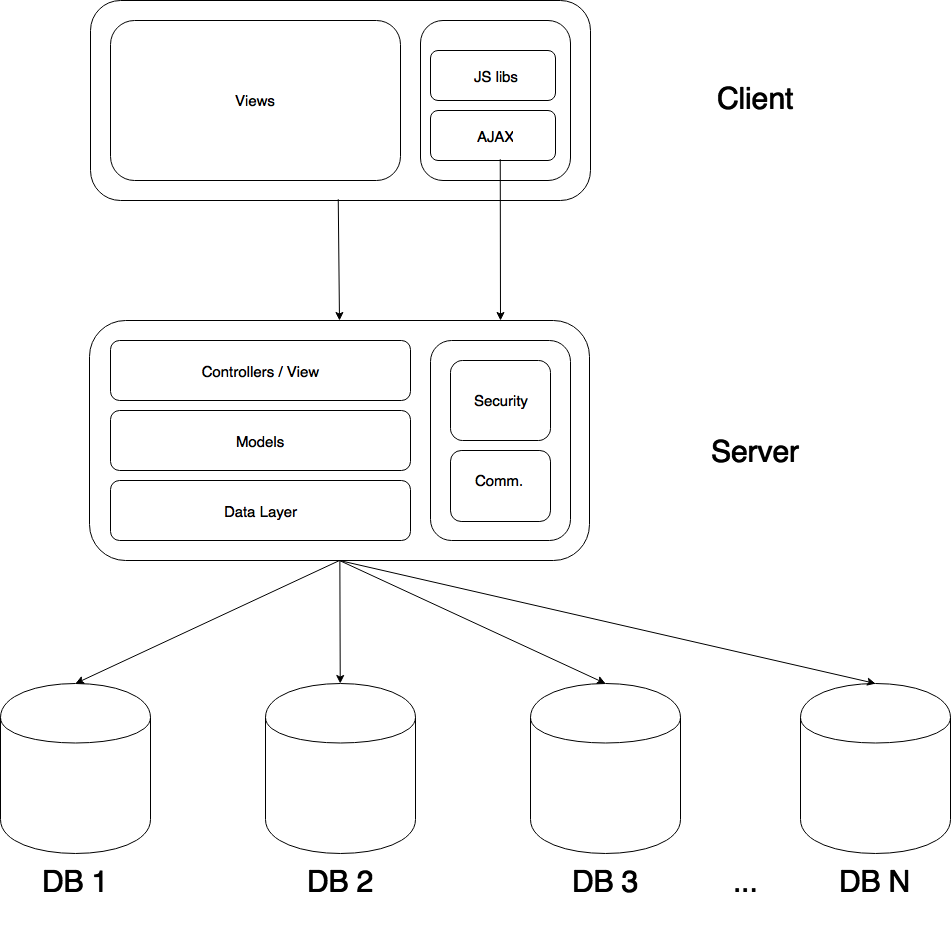
\includegraphics[width=0.6\textwidth]{architecture_1}
    \caption{The 3-tier architecture used in PitchHub capturing the security and distributed requirements identified in Chapter \ref{C:requirements} in the design.}
    \label{fig:architecture_1}
\end{figure}

\section{System Model}\label{S:systemModel}

The design of the system's model is another case of requirements being captured early in the design phase. Figure \ref{fig:class_diagram} illustrates the system's classes and their relationships as a class diagram. The requirement to implement privacy controls is captured in the Pitch Card and Comment classes' relationship with the DisclosureScope class. To illustrate this it is important to understand how the platform works: A user creates a Pitch Card, detailing the idea's attributes in the Pitch Card's Pitch Points, their aim is to get the community to collaborate on the Pitch Card to derive meaningful information or connections to action the Pitch Card, collaborator's on a Pitch Card can make suggestions or comments on these Pitch Points to help drive the idea forward. By providing scoping on Pitch Cards initiator's set a base restriction level for the Pitch Card and it's related content. The negotiation aspect of PitchHub is introduced with the Comments and Suggestions users may contribute to PitchCards. As seen in Figure \ref{fig:class_diagram} these classes also have scoping, however in this case scoping can only be set to an equivalent or more restrictive level than that specified in the Pitch Card. An example of this is where an initiator set's the content scope to `Members', so only members of the PitchHub can view the idea, now if a user were to contribute a suggestion on a Pitch Point this suggestion can only be scoped as `Members' or any level which is more restrictive, they cannot however set it to `Public'. This interaction/requirement as seen in Figure \ref{fig:class_diagram} is designed with the strategy pattern so that future scopes will have minimal change to the application.
 
\begin{sidewaysfigure}[ht]
    \centering
    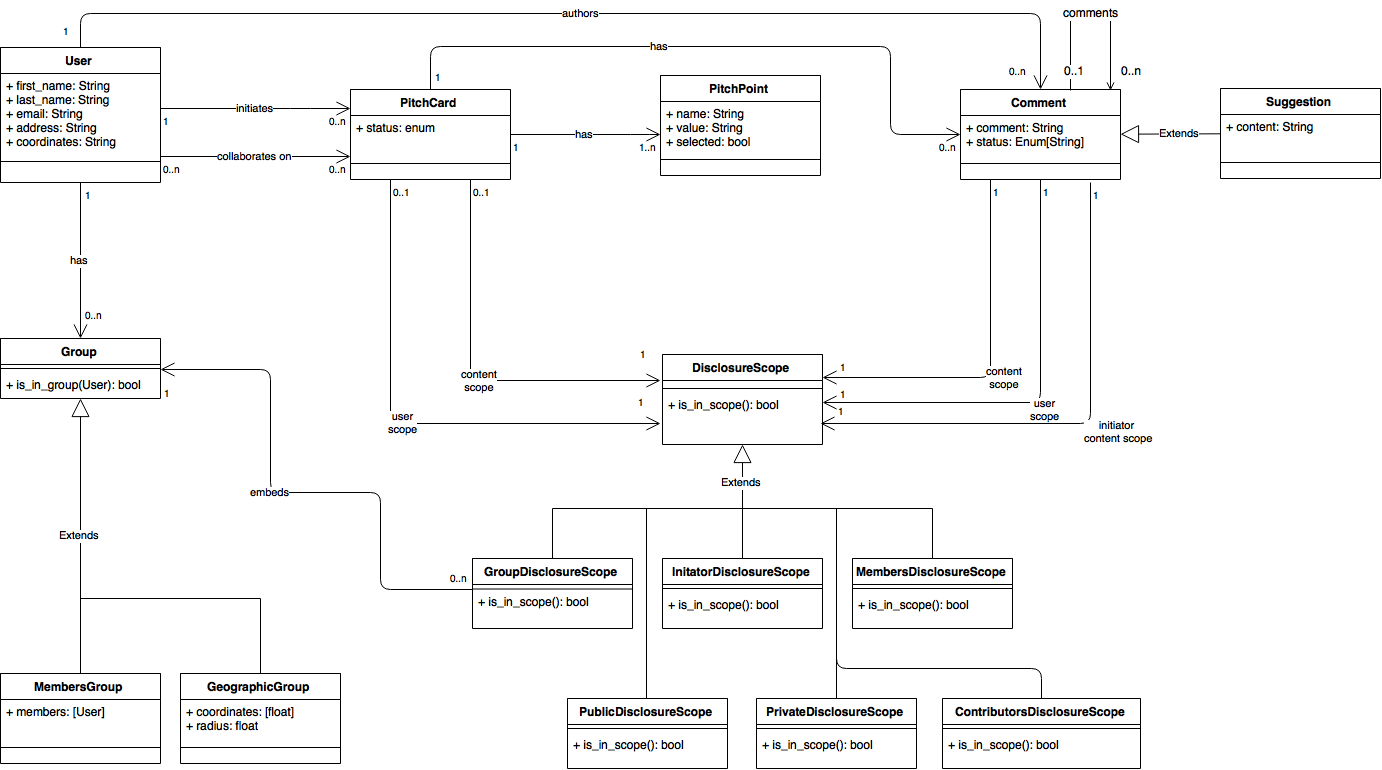
\includegraphics[width=1\textwidth]{class_diagram}
    \caption{PitchHub's system structure as represented in a class diagram. Of note is the Pitch Card and Comment classes and their relationship to the DisclosureScopes. This relationship describes the Pitch Card and Comment classes ability to scope the visibility of their content. (NB: Some attributes were left out for the sake of brevity e.g. Pitch Cards have an `images' attribute)}
    \label{fig:class_diagram}
\end{sidewaysfigure}

\section{Technology}

The quality of service attributes of a web application are deeply influenced by the fundamental technologies backing the solution. In this section both the framework and database selections are discussed in relation to quality of service attributes and more importantly the requirements identified in Chapter \ref{C:requirements}.

\subsection{Framework Selection}\label{SS:frameworkSelection}

Research was conducted on the web application frameworks available in effort to speed up the prototyping process. Ruby on Rails, Laravel, Django, MEAN and OpenSocial were identified as frameworks that could work in fulfilment of the requirements specified. Ultimately the choice of frameworks was between Ruby on Rails and OpenSocial as these were identified as being the most accessible. Ruby on Rails is an open source framework that embraces RESTful web service design and conforms to the MVC architecture. Of note, Ruby on Rails has a wealth of open-source secret sharing and functional testing libraries that are directly applicable to the requirements of this project. OpenSocial in contrast to Ruby on Rails is first and foremost a framework for creating social networks, and while PitchHub is not specifically a social network it's primary objective is to facilitate social interaction. Using OpenSocial would offer user authentication as well as messaging and posting functionality out of the box. 
\par
Of these frameworks Ruby on Rails was selected because of its vast open source library and elegant handling of complex user interaction flows. This decision results in a trade off in performance. Even in the current versions of each language Java has a significant  performance advantage over Ruby \cite{Perfo1:online}. For a simple web application this generally would not be a concern, however the secret sharing component entails the use of encryption algorithms which are computationally expensive. This was concluded not to be a major issue as Ruby on Rails offers the ability to run JRuby which is Ruby executed atop the JVM. JRuby offers significantly improved performance and even allows native Java to be executed if necessary \cite{Jruby:online}.

\subsection{Database Selection}\label{SS:databaseSelection}

The choice of database has profound effects on the performance and scalability requirements identified in Chapter \ref{C:requirements}. The rise of NoSQL databases has been attributed to the increasing need for highly scalable and performant databases. Given this need in PitchHub, in addition to PostgreSQL (Postgres), the NoSQL databases MongoDB and Cassandra were also investigated.
\par
The nature of the Pitch Card data PitchHub is modelling is inherently hierarchical and heterogeneous. In PitchHub, each Pitch Card has a varying number of Pitch Points, and each Pitch Point value also contains a number of interaction attributes. This data model naturally lends itself to the document model offered by MongoDB. Pitch Cards may be modelled in a single document with Pitch Point relations expressed via embedding. This has the additional benefit of being able to efficiently query this Pitch Cards.
\par
The case for using a relational database like Postgres is also motivated by the inherent nature of PitchHub's data. For example, each user is associated to the Pitch Cards they have initiated and contributed to, as well as the suggestions and comments they have offered on Pitch Cards. Unlike the internal model of Pitch Cards these relations are not well suited to being hierarchical as these relations have associations which are N:M rather than 1:1 or 1:N. Modelling these objects separately in tables and querying them through joins in the relational model is the ideal way to represent and query these relations.
\par
Ultimately both databases were selected for PitchHub. MongoDB has been configured as the default database in the prototype. While Postgres has been used to diversify the threshold scheme's secret keepers, this is discussed in Section \ref{SS:diverse_secret_keepers}. MongoDB was chosen as the default because the Pitch Card data is well suited to MongoDB's data model and the use case flows which require joins at most only need one join operation. It was concluded that using MongoDB and performing manual joins within the application is not a major issue because of this. Also MongoDB's ability to scale horizontally easily without the expensive migrations characteristic of relational databases provides an edge over Postgres in meeting the scalability requirement.

%!TEX root = proj_report_outline.tex
\chapter{Web Application Implementation}\label{C:webApplicationImplementation}

\section{Implementation Details}
The standard web application functionality required within the prototype, such as authentication, request life-cycles and password resets, was straightforward as Ruby on Rails solves many of these problems, and offers a wealth of libraries that can assist. The Pitch Card functionality and scope of disclosure functionality described in the Sections \ref{C:requirements} and \ref{C:design_web} were implemented from the ground up. In this Section these two functionality item's implementation details are explored.

\subsection{Pitch Card System}
As exemplified in Section \ref{C:requirements} Callaghan Innovation's specification for how the Pitch Card system works was quite mature and detailed. At it's core it required that users be able to initiate Pitch Cards and browse Pitch Cards, with the further ability to contribute suggestions or comments. To do this the web application separates the action's responsibilities. As discussed in Section \ref{SS:frameworkSelection} Ruby on Rails is architected on the MVC architecture pattern. Following Ruby on Rails convention the PitchHub prototype has models, views and controllers for each resource. The controllers adhere to the RESTful design principles, where resources are accessed using conventional HTTP resource methods and relationships are expressed via resource-nesting. The models, as designed in Figure \ref{fig:class_diagram}, were implemented with the Mongoid \cite{Mongo4:online} Object Document Mapper (ODM) for MongoDB. The Mongoid ODM subscribes to the ``convention over configuration'' philosophy that is held highly in the Ruby on Rails framework, offering a simple façade over the MongoDB query language. The views were implemented with HTML, SASS (CSS), and JavaScript. To enhance the user experience AJAX was implemented to speed up page load times by loading secondary or non-essential data asynchronously. AJAX was also heavily used in user interactions, such as contributing a suggestion/comment and setting disclosure scopes (as an initiator).
\par
Figure \ref{fig:pitch_card_pitchhub} showcases the prototype's Pitch Card view from the initiator's perspective. The view can be deconstructed as follows: the sidebar contains the links to the main pages, the navigation bar contains the search box and user management drop-down, the main page space contains the Pitch Card and it's associated suggestions. Figure \ref{fig:dashboard_pitchhub} contains the same sidebar and navigation bar however the main page space contains a grid of mini-pitch card views consisting of the Pitch Card's image (if any) as well as the \textit{Value Proposition} pitch point.

\subsection{Scope of Disclosure}
As previously discussed in Section \ref{S:systemModel} and shown in Figure \ref{fig:class_diagram} the scope of disclosure functionality is implemented on both Pitch Card and Suggestion/Comment models. For Pitch Cards this scope of disclosure is achieved through a combined effort at the database level and at the application level. To illustrate this consider the \ref{fig:dashboard_pitchhub}. When the user loads up the dashboard the database is queried asking for Pitch Cards that the current user is able to see (if any). How this first step works is through the use of MongoDB's aggregation pipeline \cite{Aggre7:online}. The aggregation pipeline in this instance deals with the fact that users assume different roles in the context of different Pitch Cards, and Pitch Cards themselves are heterogeneous in the scopes they are defined with. Unlike role-based Access Control Lists, where a user is checked if their role satisfies a particular permission level, the pipeline designed for PitchHub checks the user against each role of the Pitch Card and then against the Pitch Card's visibility scope. This single pipeline aggregation query basically checks a matrix of constraints to check each context. This is visualised in Figure \ref{fig:pipeline}.

\begin{figure}[ht]
    \centering
    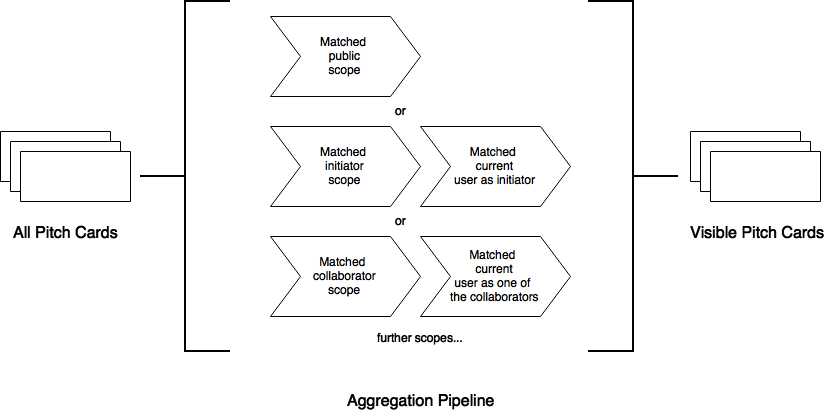
\includegraphics[width=1\textwidth]{pipeline}
    \caption{The pipeline aggregation query used to find all visible Pitch Cards checks for the scoping of the Pitch Card from the context of the current user.}
    \label{fig:pipeline}
\end{figure}

Continuing the example above, once the viewable Pitch Cards for the Dashboard view have been retrieved from the database the application applies the identity scopes for each Pitch Card in the view. This piece of functionality decides whether the the initiator will appear by their name or by `anonymous'. The way this is implemented is made simple through the ODM, where when the Pitch Card object is retrieved, the Pitch Card's nested scope objects are also retrieved. As seen in Figure \ref{fig:class_diagram} these scope objects implement the strategy pattern, so when they are retrieved the application is able to easily check whether the current user is authorised to see the Pitch Card's author agnostic of the actual scope being used. The use of the strategy pattern removes the need to do the less-pragmatic and less-extensible type-checking on scope objects to determine what scoping business logic should be used.
\par
The marriage of database-level and application-level scoping caters to the context of the request's life-cycle stage to maximise efficiency. Certainly, it would have been possible to use the strategy pattern object scoping instead of what is essentially type-checking in the aggregation pipeline query to achieve this scoping. However, at this point in the request the application does not have Pitch Card objects (and their nested scope objects) to scope by, therefore by expressing this logic in the database query the application is able to appropriately apply scope given the context, retrieving only the viewable Pitch Cards.

\section{Implementation Challenges}

\subsection{Virtualised Environment}
The time-constrained weekly/bi-weekly meetings with Callaghan Innovation elicited the need for their own locally hosted PitchHub instances. Their own PitchHub instances enabled them to check the progress of the prototype, answer UI/UX questions, and show the prototype to other Callaghan Innovation personnel. 
\par
Personally configuring the environment and setting up PitchHub was an option, however this would have still been a lengthy process detracting from actual meeting. Furthermore it would have been infeasible to repeat this for each stakeholder and their various machines. Requiring the stakeholders to do this themselves would have similarly been infeasible as configuring a locally hosted Ruby on Rails application is a non-trivial task \cite{Roma:personalCommunications}, to exemplify this StackOverflow has excess of 50,000 questions in relation to Ruby on Rails installation/configuration \cite{StackOverflowProblem1:online, StackOverflowProblem2:online, StackOverflowProblem3:online, StackOverflowProblem4:online}.
\par
To solve this problem the PitchHub environment and installation process was automated using a combination of Chef and Vagrant scripts. Vagrant was employed to automate the Ubuntu virtual machine setup and Chef was leveraged to manage PitchHub's various environment dependencies (Ruby, a JS runtime, and MongoDB). By having this infrastructure/configuration implemented via code it also serves as documentation for the PitchHub environment and enables the use of version control within this aspect of the project. This process has the further advantage in that any future contributors to the project will have a very low barrier to entry in terms of setting up their own locally hosted PitchHub instance.

\subsection{Deployment}
As discussed in Section \ref{S:projectObjectives} one of the objectives was to have a prototype deployed by August so that Callaghan Innovation may conduct an internal user study. The deployment process of PitchHub consisted of two steps: first, setting up the infrastructure for the deployment and second, deploying the Ruby on Rails prototype onto the infrastructure. To support the first step, Callaghan Innovation provided a machine, racked it in their server room, and also configured the machine's domain name. I then completed the infrastructure setup by configuring the nginx HTTP server \cite{nginx2:online}, the Phusion Passenger application server \cite{phusionPassenger:online} and SSL. In regards to step 2, there exist a few prominent methods of deploying Ruby on Rails applications:
\begin{itemize}
    \item A manual process using a combination of SFTP and SSH, to transfer files and update environment variables.
    \item An automated process facilitated by Capistrano, a Ruby on Rails deployment library.
\end{itemize}

The manual process, while easier for the initial deployment, was decided against as the process is brittle in that it relies on the deployer to fulfil each deployment step correctly and in order. For a Ruby on Rails application this process at the very minimum consists of: transferring the updated application code, pre-compiling the assets, downloading any newly added libraries and updating the binaries. Should this be done incorrectly or in the wrong environment this manual process has no `undo' action, therefore the process of reverting the application must also be done manually. Capistrano alleviates these problems but at the cost of a steep-learning curve. Capistrano is similar to Vagrant in that the process is automated by scripts which automate the entire process. Ultimately, the initial investment in defining the scripts is negligible in comparison to the long term gains of robust and consistent deployments. PitchHub is currently hosted at \textit{pitchhub.net}, note that the current release is being used internally in Callaghan Innovation and requires an access code to sign up.

\begin{sidewaysfigure}[ht]
    \centering
    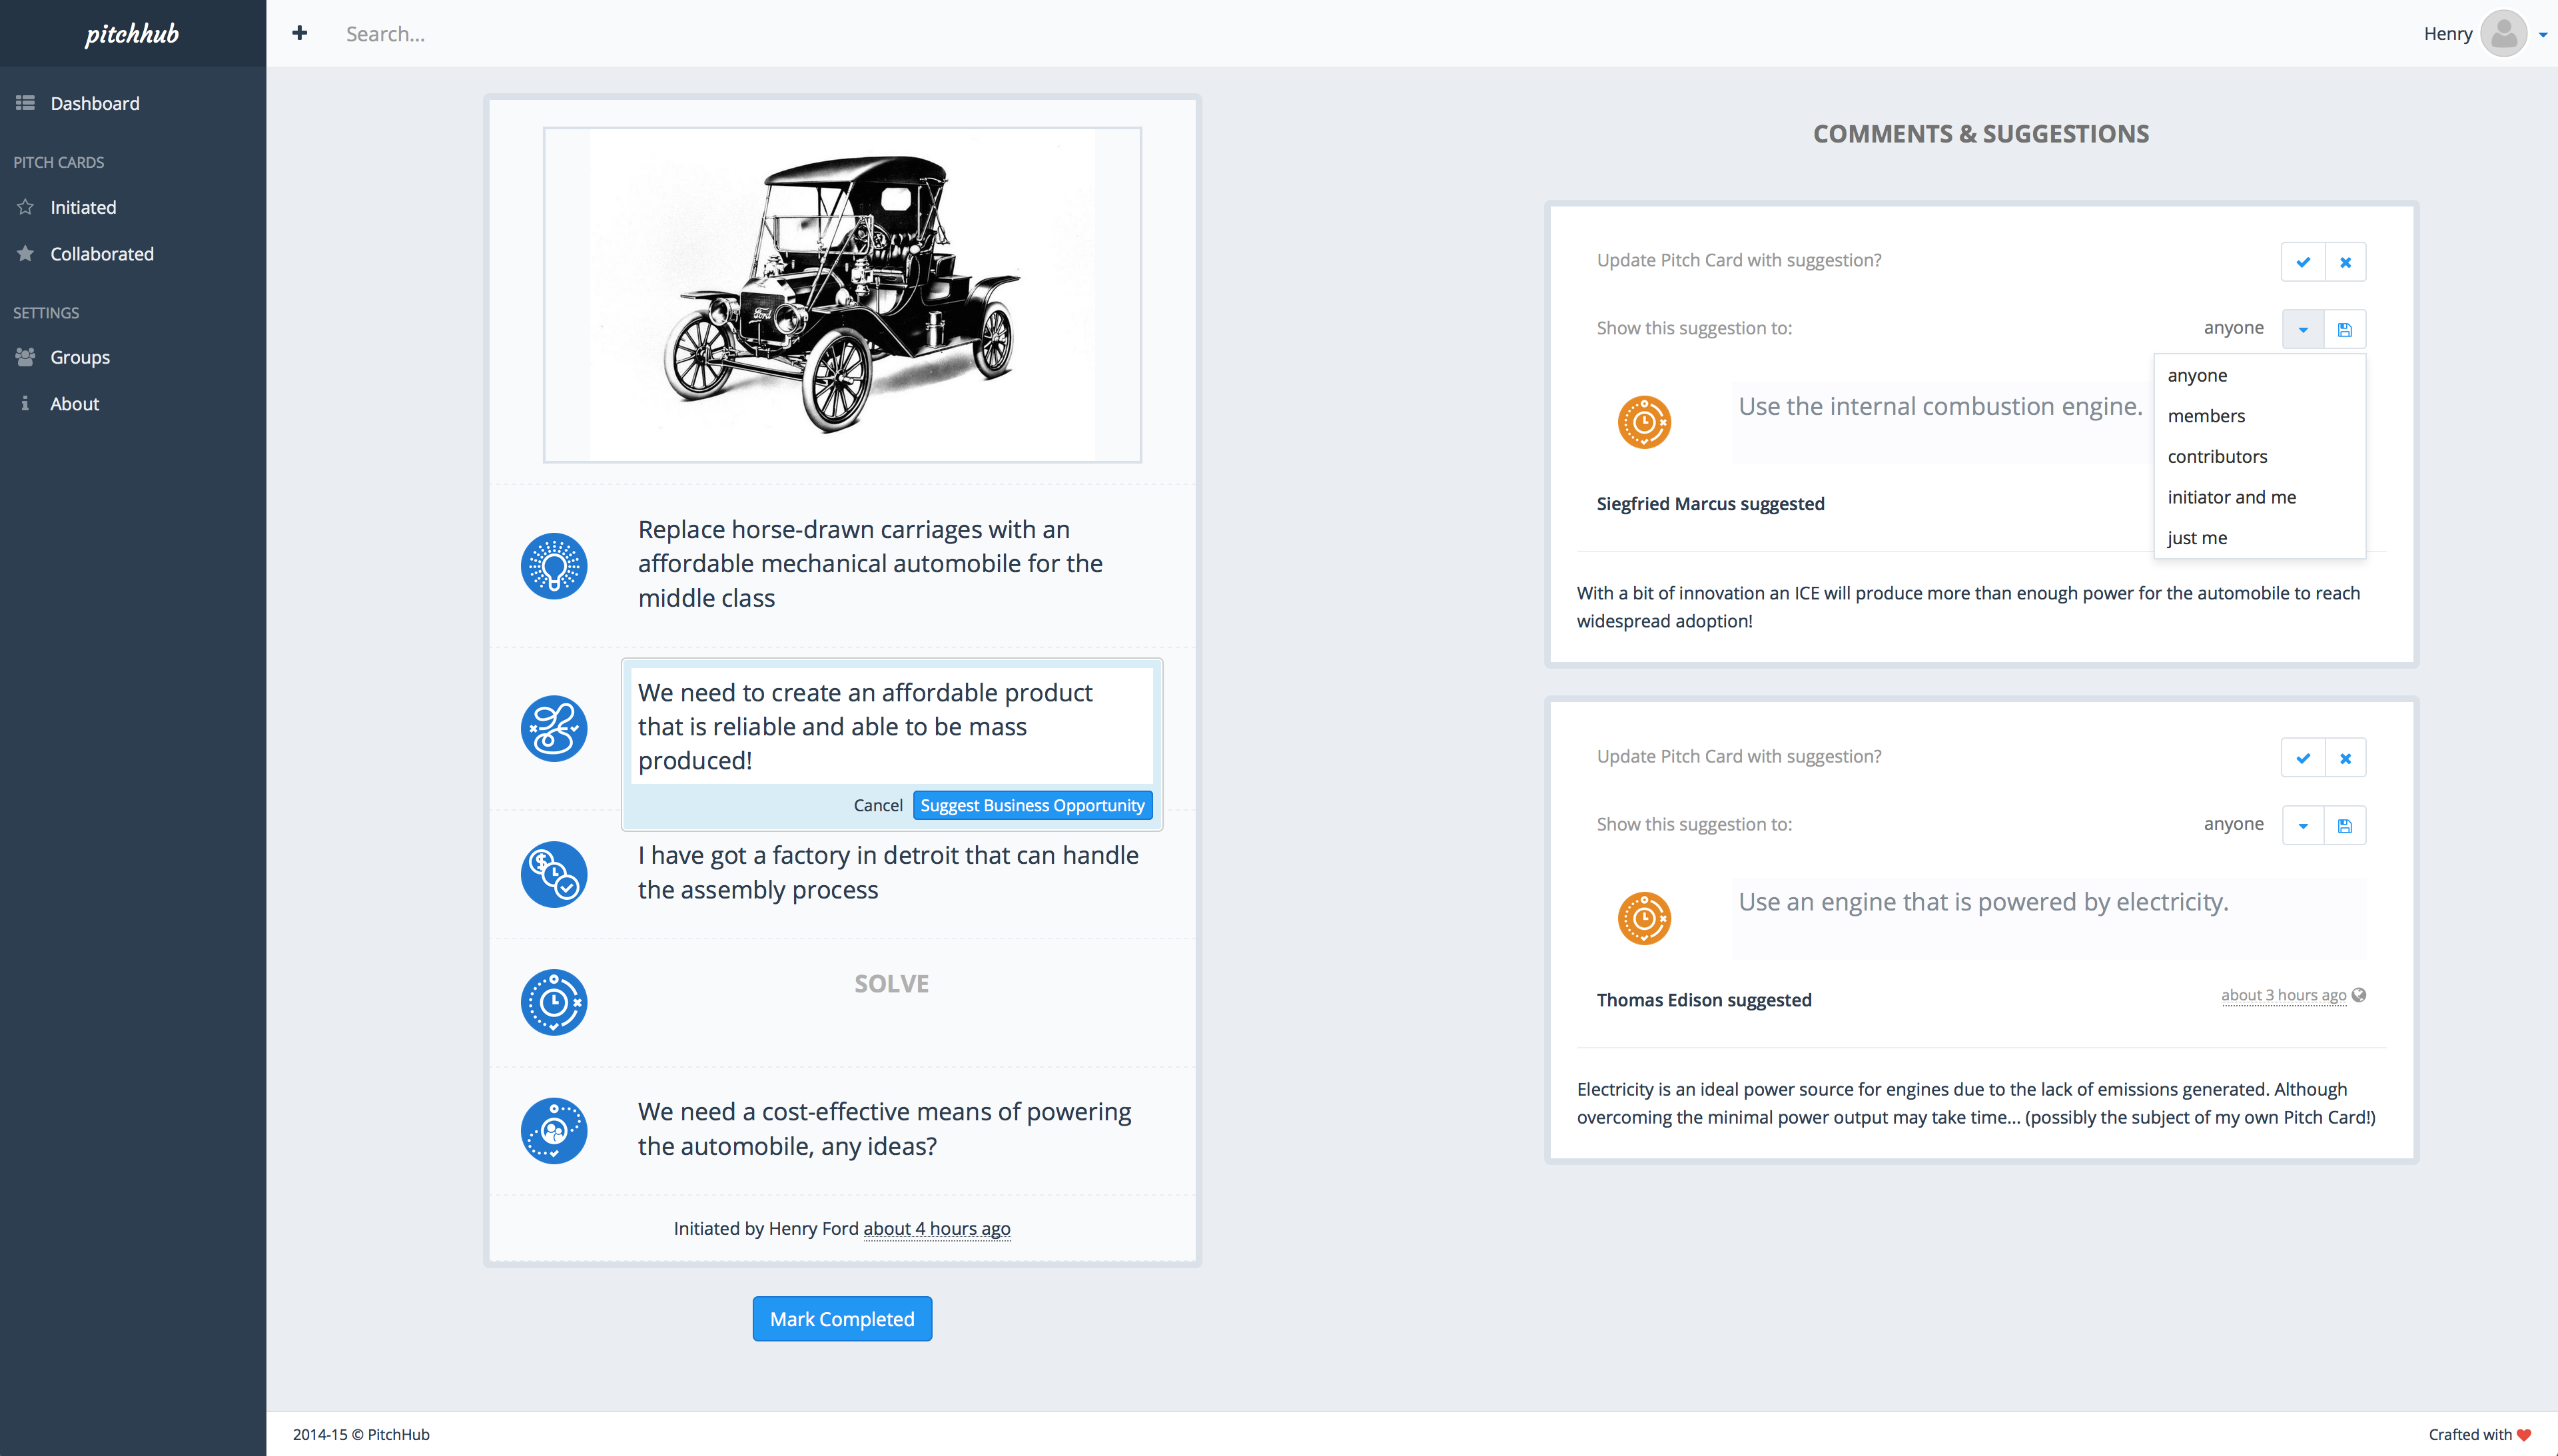
\includegraphics[width=1\textwidth]{pitch_card_pitchhub}
    \caption{Fictional Ford Model T Pitch Card view from the initiator's perspective. The view is divided into two sections the Pitch Card and it's suggestions/comments. In the Pitch Card half users perform in-line editing on a Pitch Point to make a suggestion. In the suggestion/comments half the initiator may accept or decline the suggestion and set the suggestion/comment's scope.}
    \label{fig:pitch_card_pitchhub}
\end{sidewaysfigure}

\begin{sidewaysfigure}[ht]
    \centering
    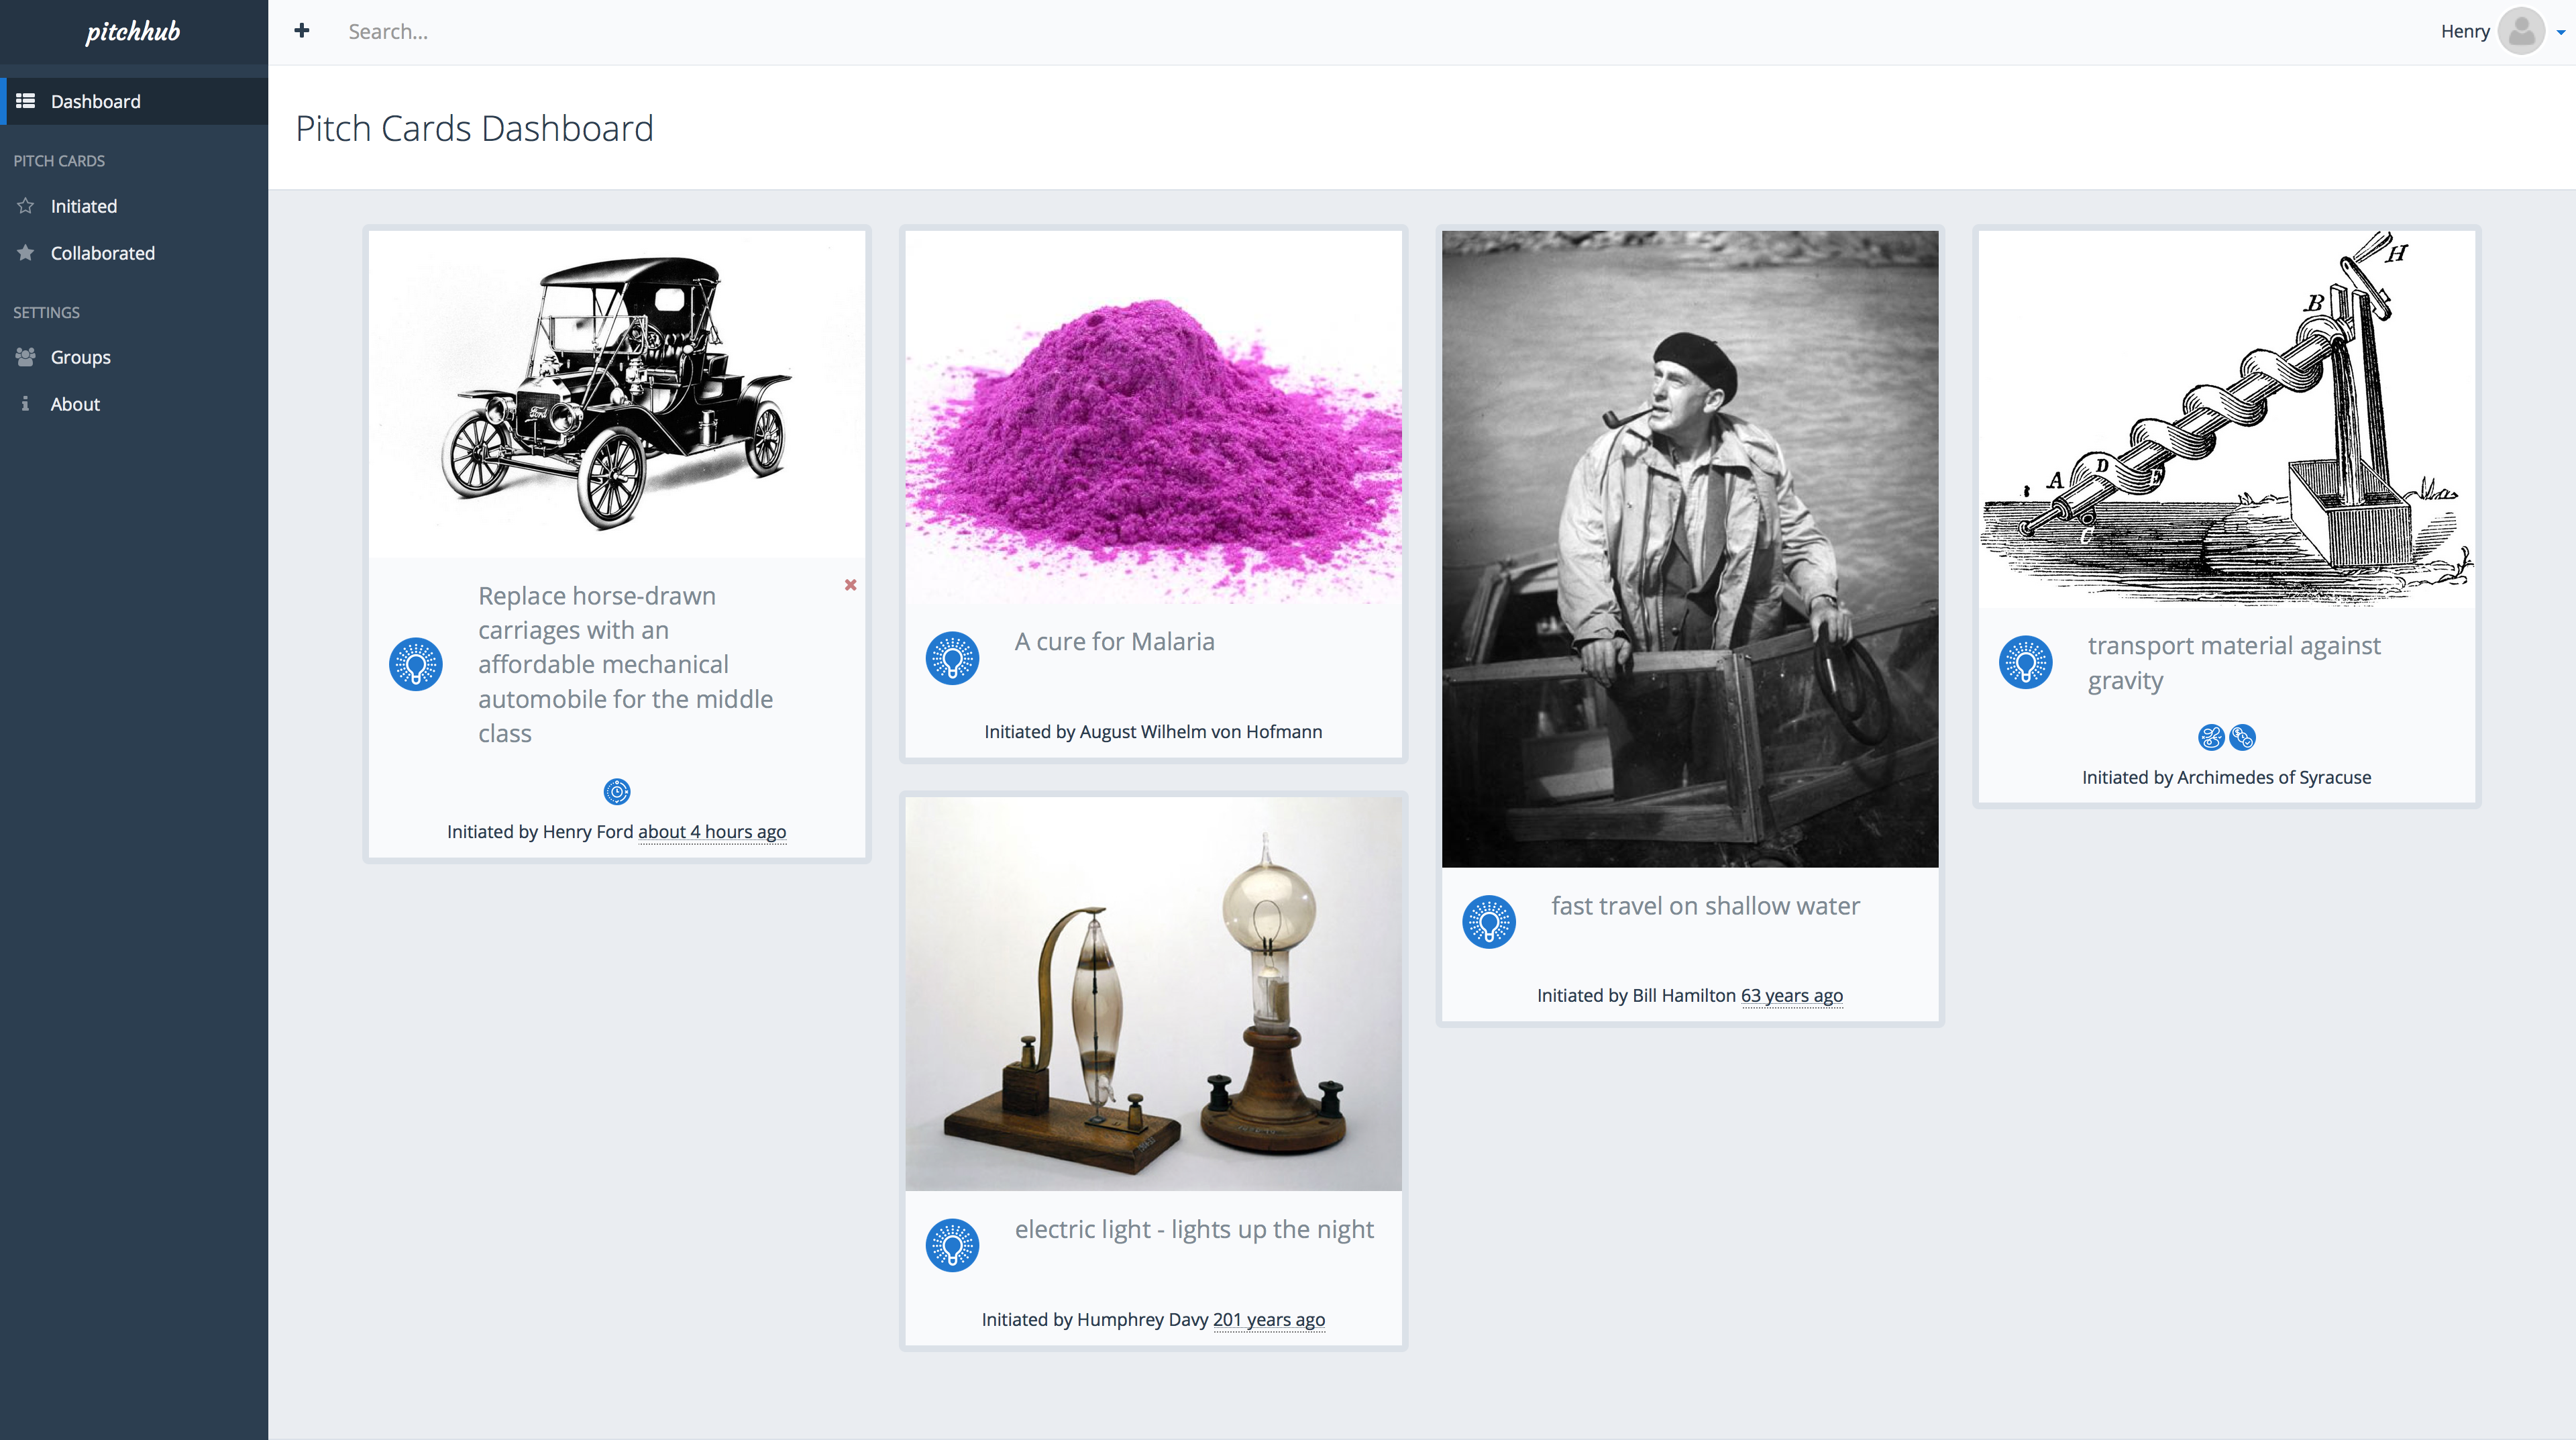
\includegraphics[width=1\textwidth]{dashboard_pitchhub}
    \caption{PitchHub's dashboard populated with fictional Pitch Cards. The grid layout displayed is responsive, so the Pitch Cards will reorganise and size to fit the user's device screen.}
    \label{fig:dashboard_pitchhub}
\end{sidewaysfigure}
%!TEX root = proj_report_outline.tex
\chapter{Background into the Threshold Security Scheme}

\section{Security Considerations}

\section{Shamir's Secret Sharing Scheme}

\section{Limitations of Threshold Security Schemes}
\chapter{Implementation of the Threshold Security Scheme}

\section{Implementation of Shamir's Secret Sharing Scheme}

\section{Implementation of Secret Keeper Redundancy}
%!TEX root = proj_report_outline.tex
\chapter{Experimental Methodology}

\section{Functional Testing Method}

\subsection{Testing Environment}

talk about reproducible environment

\subsection{Test Data}

frequency analysis of data cleaned and given by CI's user trial

seeded given frequency analysis results

\subsection{Automated Testing}

talk about selenium and user stories

\subsection{Performance Considerations}

talk about NN threshold

\section{Security Testing Method}

\subsection{Security Testing Scope}

Our threat model consists of resisting at least one shoulder surfing attack from an observer co-located at any position around the tabletop. Camera-based attacks are feasible with most knowledge-based authentication systems; but to defeat camera attacks was not our design goal. The pervasive na- ture of mobile devices instrumented with cameras is of par- ticular concern, but as with other manifestations of this same problem (e.g. at the ATM) we rely upon social conventions to deter active attempts to video record logins.

\subsection{Threat Taxonomy}
%!TEX root = proj_report_outline.tex
\chapter{Evaluation}

\section{Functionality}

\subsection{User Stories}
To evaluate whether the requirements D1, D2.1 and D2.2 have been fulfilled, the system's behaviour was tested in regards to each of these requirements. 
Requirement D1's user stories specify the ability to post Pitch Cards, make suggestions on Pitch Points, accept/reject Pitch Points, comment on Pitch Points, comment on suggestions and mark Pitch Cards as completed/active. 

Requirement D2.1's user stories specify the ability to scope entities such as Pitch Cards, Suggestions, and one's identity such that unintended viewers are avoided. To ensure the completeness of these scope tests these user stories were derived from the following behaviour matrix:

\begin{figure}[ht]
    \centering
    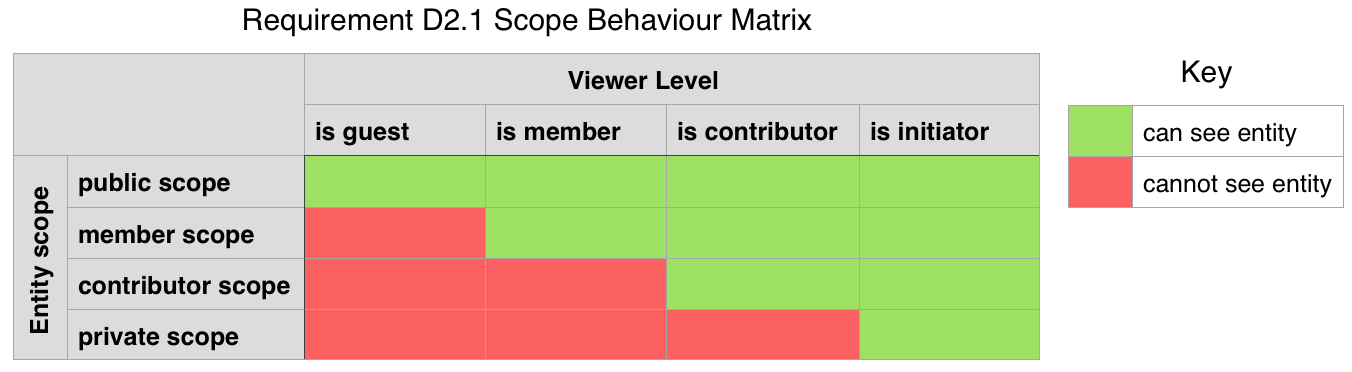
\includegraphics[width=1\textwidth]{scope_matrix}
    \caption{The scope matrix which illustrates the relationship between user level and entity scope in regards to viewing the entity.}
    \label{fig:architecturescope_matrix_evaluation}
\end{figure}


Requirement D2.2's user stories specify that users who have viewed a Pitch Card are able to be seen as a ``viewer'' by the initiator.

Given that these user stories are verified as working by \textit{TB3} it is concluded that requirements D1, D2.1 and D2.2 have been fulfilled.

\subsection{Deployed Prototype}
At the time of writing, the prototype has been successfully been deployed to Callaghan Innovation and is ready for use. Unfortunately use of the prototype by Callaghan Innovation has not yet fully commenced. Without substantial activity to analyse this component of the evaluation was unable to be completed. It is expected that the access code will be distributed by the Callaghan Innovation stakeholders to the wider organisation in the coming weeks.

\section{Performance}

\subsection{Nielsen's Response Time Thresholds}

\subsection{Test 1 - User Size}

\subsection{Test 2 - Overhead of Threshold Scheme Security}

\subsection{Test 3 - Overhead of Secret Keeper Diversity}

\subsection{Discussion}

A limitation of the experiment described in Section \ref{SS:performance} is that it is only semi-globally distributed. Two servers hosted on AWS (located in Oregon, USA) and two servers hosted by Callaghan Innovation in Wellington provide an uncommon network topology. The Secret Sharing Service with the ``3, 4'' threshold scheme means that on each database query at least one request will be sent to one of the AWS instances. This impacts the performance results due to the latency incurred. For performance results it would have been better to have all servers hosted within New Zealand. However, security and disaster recovery considerations motivated the move to embrace a more geographically distributed network.

The disadvantage of unconditionally secure secret sharing schemes is that the storage and transmission of the shares requires an amount of storage and bandwidth resources equivalent to the size of the secret times the number of shares. If the size of the secret were significant, say 1 GB, and the number of shares were 10, then 10 GB of data must be stored by the shareholders

%!TEX root = proj_report_outline.tex
\chapter{Conclusions and Future Work}
This chapter reviews the project's contributions in light of the design requirements, discusses potential future work and finally, surmises the project.

\section{Review}

The project's principal contributions are as follows:

\paragraph{C1:} I have developed an {\em Innovation Role Taxonomy} for classifying existing innovation platforms. The relationship semantics between roles in the taxonomy is denoted as either explicitly supported or implicitly supported. Platforms that facilitate innovation collaboration ideally have explicit support for all roles.

\paragraph{C2:} I have designed a {\em new UI} to encourage collaboration and be visually appealing. Content templates and wire frames were key artefacts produced to guide the final implementation.

\paragraph{C3:} I have designed the {\em PitchHub distributed architecture}. The tiered architecture style adopted supports ease of extension for future development.

\paragraph{C4:} I have developed {\em the first suite of user stories} that capture the interactions of innovation collaboration. These stories specify the following: engagement of all roles within the innovation community, the ability to scope content's disclosure, and audit who has seen ideas that you have initiated.

\paragraph{C5.1:} I have implemented the {\em PitchHub prototype}, a platform that supports the innovation collaboration user stories specified. Built on the popular Ruby on Rails framework and good coding practices this artefact is open to future development.

\paragraph{C5.2:} I have {\em deployed a PitchHub prototype} to Callaghan Innovation for their use. This instance contains the following production configuration: a Passenger application server, caching, SSL, and various security measures suggested by OWASP (e.g. ssh hardening, protection against IP spoofing). Visit \url{http://pitchhub.net} to view this instance.


\paragraph{C5.3:} I have implemented a {\em PitchHub prototype with Shamir's Secret Sharing scheme} integrated. Sensitive information such as Pitch Points, suggestions, and comments is encrypted using this service.

\paragraph{C5.4:} I have implemented a {\em PitchHub prototype with diverse secret keepers} to strengthen the security provided by the Secret Sharing scheme. The prototype supports the following databases: MongoDB, Postgres, MySQL and SQLite. To maintain the \textit{plug-and-play} functionality afforded by MongoDB the configuration required by SQL secret keepers has been automated.

\paragraph{C6:} I have virtualised the {\em PitchHub development environment} using Vagrant and Chef to make installation and setup of PitchHub as easy as possible. This was primarily for the benefit of non-technical stakeholders, but will be equally useful for future maintainers.

\paragraph{C7:} I have automated the {\em PitchHub deployment process} using Capistrano to make host configuration and code deployment as easy as possible. The scripts defined facilitate zero-downtime deployments and also enable deployments to be rolled-back easily.
\\
\newline
These contributions are instrumental in fulfilling the design requirements identified in Section \ref{S:designRequirements}. The fulfilment relationship between contributions to requirements is shown in Fig \ref{fig:contribution_requirements_mapping}.

\begin{figure}[ht]
    \centering
    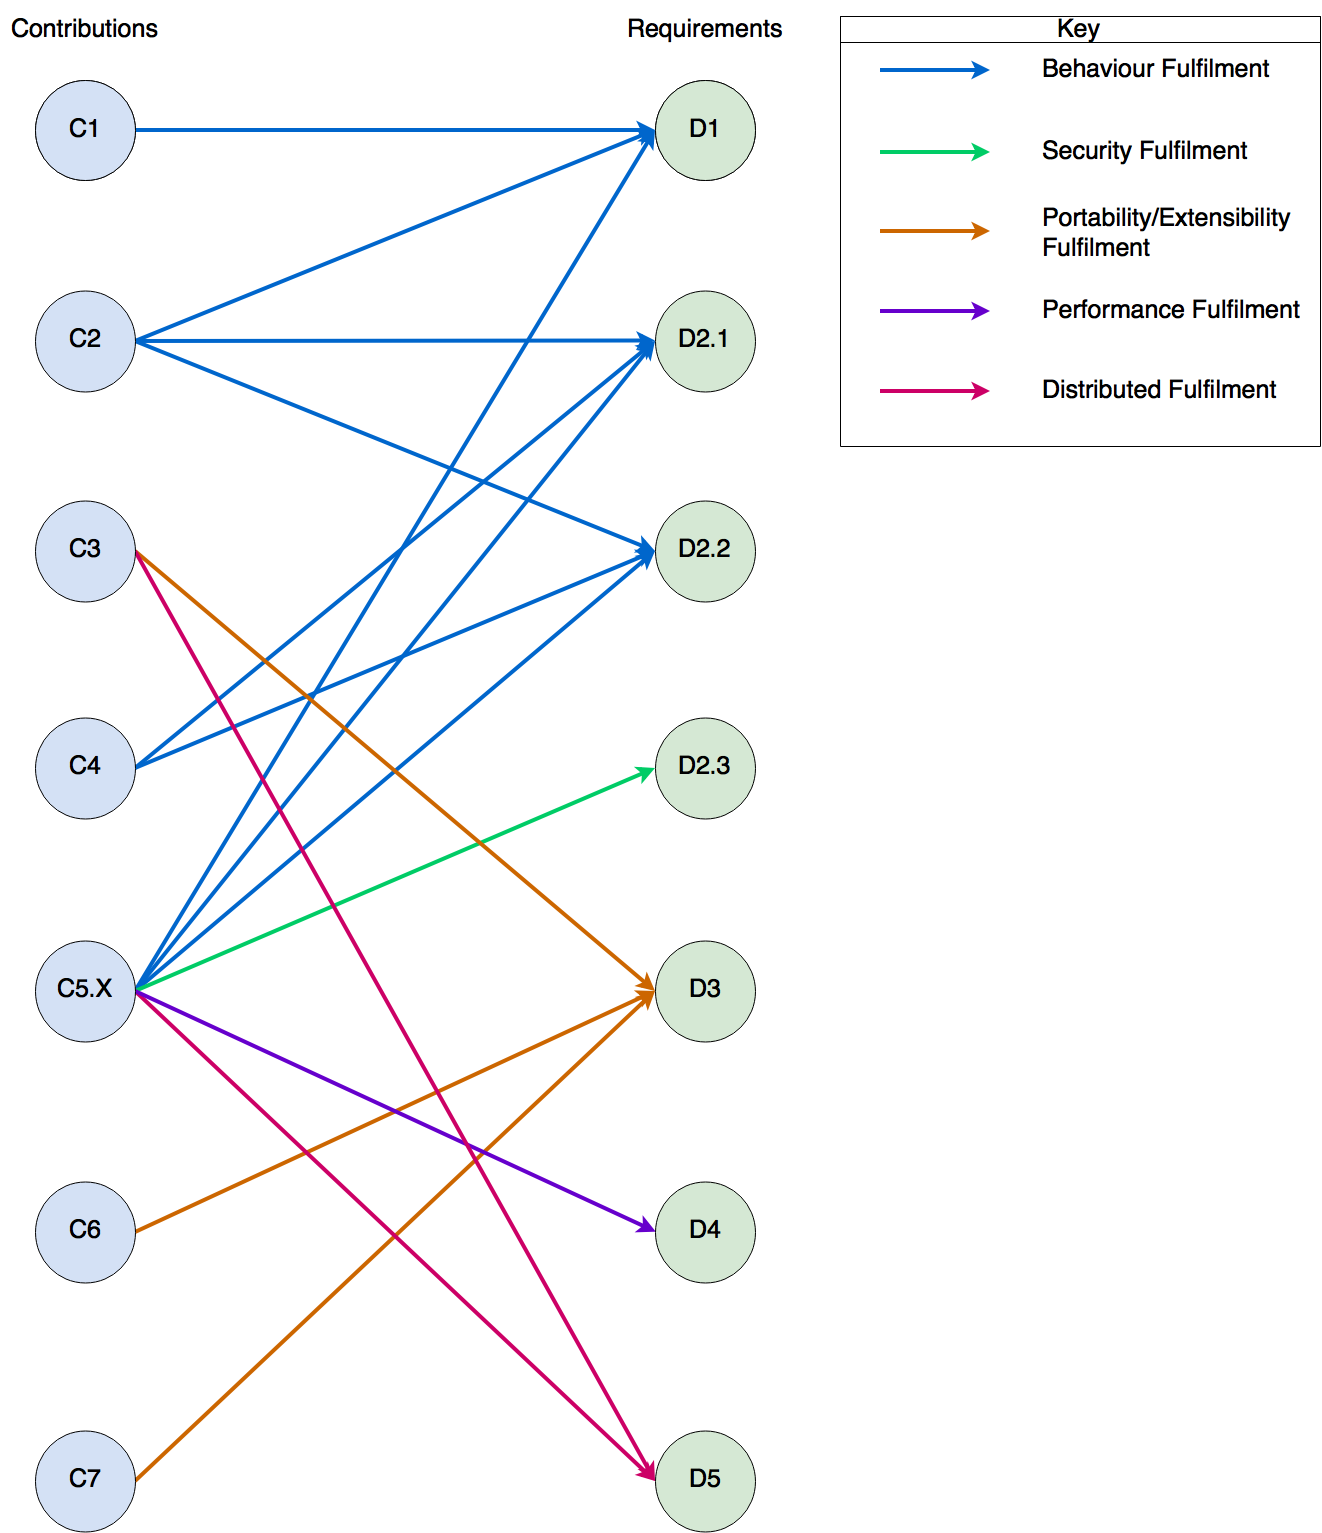
\includegraphics[width=0.65\textwidth]{contributions_requirements_map}
    \caption{A mapping of contributions to requirements denoting fulfilment.}
    \label{fig:contribution_requirements_mapping}
\end{figure}

C2, C4, and C5.{\em X} all play roles in the fulfilment of requirements D1, D2.1, and D2.2. The user stories created in D1 capture the behaviours required by D1, D2.1, and D2.2. These user stories were used to drive the design process of the UI (C4) that C5.{\em X} ultimately uses to facilitate these behaviours. The strict adherence to the user stories throughout the design and execution of the project has culminated in artefacts that are faithful in their support of the behaviours required. This fulfilment has been verified by Test \rom{1} and thus requirements D1, D2.1, and D2.2 are concluded as fulfilled.

C5.3 and C5.4 contribute to the fulfilment of requirement D2.3. Integrating the Secret Sharing scheme into the prototype and encrypting commercially sensitive data and IP at the Pitch Point level ensures unconditional security in relation to database breaches (of up to \textit{k}). As described in Section \ref{S:evaluationScope} verification of this component was out of scope of this project. Despite this, it is believed that requirement D2.3 has been fulfilled to the extent possible within the scope of this project.

C3, C6 and C7 each play roles in satisfying requirement D3. The architecture (C3) aids extensibility through the tiered architecture style adopted. The virtualised development environment (C6) is key in providing portability, enabling \textit{plug-and-play} functionality for all artefact prototype variations (C5.{\em X}). C7 aids in the extensibility of the deployment process, as new tasks and environment targets can be easily added.

C5.{\em X} has been used to verify the fulfilment of requirement D4 through Tests \rom{3}-\rom{6}. Specifically, Tests \rom{3}-\rom{5} verify that the main flows can be performed within Nielsen's time thresholds (in different Secret Sharing configurations) and Test 6 verifies that the prototype can sustain the expected community size's load while maintaining the mean response wall-time within the time thresholds. Therefore, in the context of Nielsen's response time thresholds requirement D4 has been met.

C3 demonstrates the distributed architecture PitchHub is built upon in satisfaction of requirement D5. Ultimately through C5.3 and C5.4's verification of C3's design in their implementation and evaluation it is concluded that requirement D5 has been satisfied.

\section{Future Work}

This section discusses potential extensions to the PitchHub prototype.

\subsection{Recommendation Engine}

A potentially useful feature would be if Pitch Cards could be recommended to users based on their ontological profile. This would encourage collaboration through showing users ideas they are more likely to have an interest in. Offline learning is certainly viable, but an interesting challenge would be integrating the recommender to work with the Secret Sharing service in an online learning approach.

\subsection{Usability Extension/Evaluation}

Future work concentrating on the usability of PitchHub could focus on evaluating and extending the current prototype. A user study would be beneficial in verifying the accuracy of the behaviours identified in the user stories. A user study could also help with the identification of new user stories and potential functionality extensions. 

\subsection{RealMe Integration}

When PitchHub is released to the public it may be open to abuse by users creating fake accounts. These fake accounts may be used maliciously to view others' IP or contribute unhelpful suggestions. Therefore it is important to for users on PitchHub to be verified as being who they say they are so that there may be a sense of accountability. A service like RealMe would be ideal for this as it is maintained by the Department of Internal Affairs and the actual identity verification process is facilitated by them. To integrate RealMe into PitchHub would require using RealMe's SAML service for authentication.
\include{8_future_work}

% \include{using}
% \include{example}

%%%%%%%%%%%%%%%%%%%%%%%%%%%%%%%%%%%%%%%%%%%%%%%%%%%%%%%

\backmatter

%%%%%%%%%%%%%%%%%%%%%%%%%%%%%%%%%%%%%%%%%%%%%%%%%%%%%%%


\bibliographystyle{IEEEtranN}
\bibliography{final}


\end{document}
